
\subsection{NiosII CPU modules description}

The CPU hardware structure is made of different modules, and every module have his scope. \\
The main modules are:

\begin{itemize}
    \setlength\itemsep{0pt}
    \setlength\parskip{0pt}
    \item \textbf{Clock modules}: Used to manage the different clock sources.
    \item \textbf{Memory modules}: Used to connect the CPU to different memories, either internal or external to the chip.
    \item \textbf{Nios II modules}: Used to instantiate the CPU module and the system ID module.
    \item \textbf{PIO modules}: Used to instantiate the I/O peripherals. 
    \item \textbf{System peripherals}: Peripherals useful for programming and debugging, such as timers or UART devices.
    \item \textbf{LT24 modules}: Different modules used to control the LT24 LCD and touch screen (see \cite{rocketboards2024}). 
    \item \textbf{Floating-point operator module}: Used to instantiate hardware multipliers, dividers, and other floating-point operators.
\end{itemize}

\subsubsection{Clock Modules}

The clock section contains the modules required to generate and distribute the system clocks. \\
The \texttt{clk\_in} module provides the external reference clock, while the \texttt{system\_pll} module generates the internal clocks required by the system. \\
The \texttt{mm\_clock\_crossing\_bridge} module is used to connect components working on different clock domains.

\begin{figure}[h!]
    \centering
    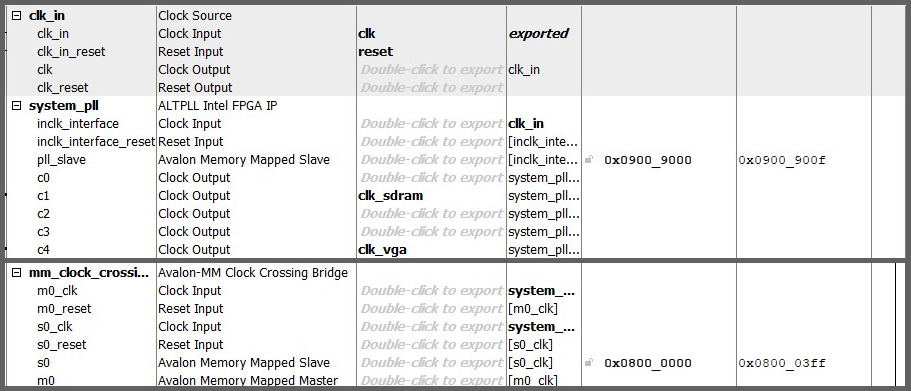
\includegraphics[width=1\linewidth]{img/clk_modules.jpg}
    \caption{CPU clock modules instantiated}
    \label{fig:clk_modules}
\end{figure}

\newpage

\subsubsection{Memory Modules}

The memory section contains the modules used for data and program storage. \\
The \texttt{onchip\_memory} module provides a small and fast internal memory, while the \texttt{sdram} module instantiate a controller for the external SDRAM memory to increase the available storage capacity.

\begin{figure}[h!]
    \centering
    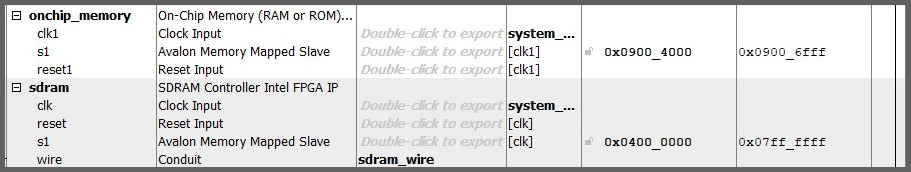
\includegraphics[width=1\linewidth]{img/memory_modules.jpg}
    \caption{CPU memory modules instantiated}
    \label{fig:memory_modules}
\end{figure}

\subsubsection{NiosII Modules}

The main processing section is based on the \texttt{nios2\_gen2} soft-core processor, which executes the software running on the FPGA. \\
The \texttt{sysid\_qsys} module is used to identify the generated system configuration and ensure software compatibility.

\begin{figure}[h!]
    \centering
    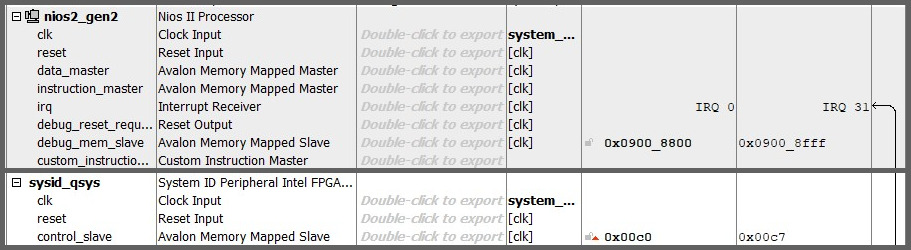
\includegraphics[width=1\linewidth]{img/nios2_modules.jpg}
    \caption{CPU (NiosII) modules instantiated}
    \label{fig:nios2_modules}
\end{figure}

\newpage

\subsubsection{PIO Modules}

The PIO modules are used to interface simple digital peripherals with the processor. \\
These modules manage input and output devices such as LEDs, switches, buttons, and other GPIO peripherals through memory-mapped registers.

\begin{figure}[h!]
    \centering
    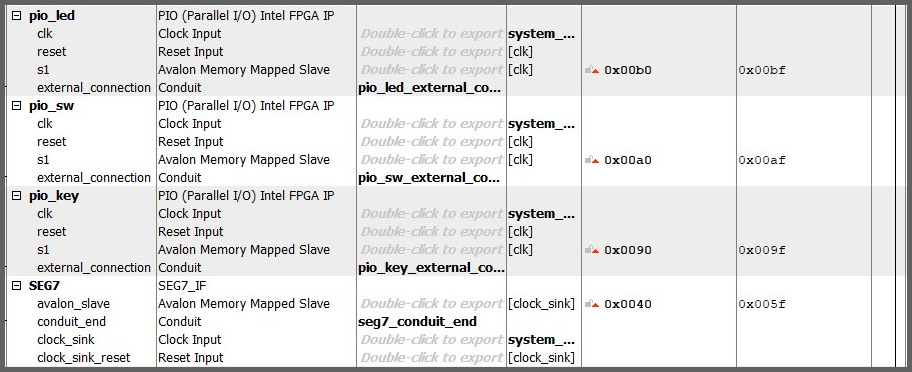
\includegraphics[width=1\linewidth]{img/pio_modules.jpg}
    \caption{CPU PIO modules instantiated}
    \label{fig:pio_modules}
\end{figure}

\subsubsection{System peripherals}

The system peripheral section contains modules used for communication and timing operations. \\
The \texttt{jtag\_uart} module allows serial communication and debugging through the JTAG interface, while the \texttt{timer} module provides timing and delay functionalities for the software running on the processor.

\begin{figure}[h!]
    \centering
    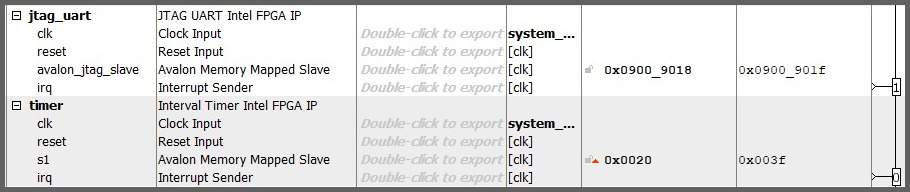
\includegraphics[width=1\linewidth]{img/system_perip_modules.jpg}
    \caption{CPU system peripherals instantiated}
    \label{fig:system_perip_modules}
\end{figure}

\newpage

\subsubsection{LT24 modules}

The LT24 section contains the modules required to control the LCD touchscreen display. \\
The \texttt{LT24\_Controller} module manages the communication with the display, while \texttt{LCD\_RESET\_N} handles the display reset signal. \\
The touchscreen interface is managed through the \texttt{touch\_panel\_spi}, \\\texttt{touch\_panel\_pen\_irq}, and \texttt{touch\_panel\_busy} modules.

\begin{figure}[h!]
    \centering
    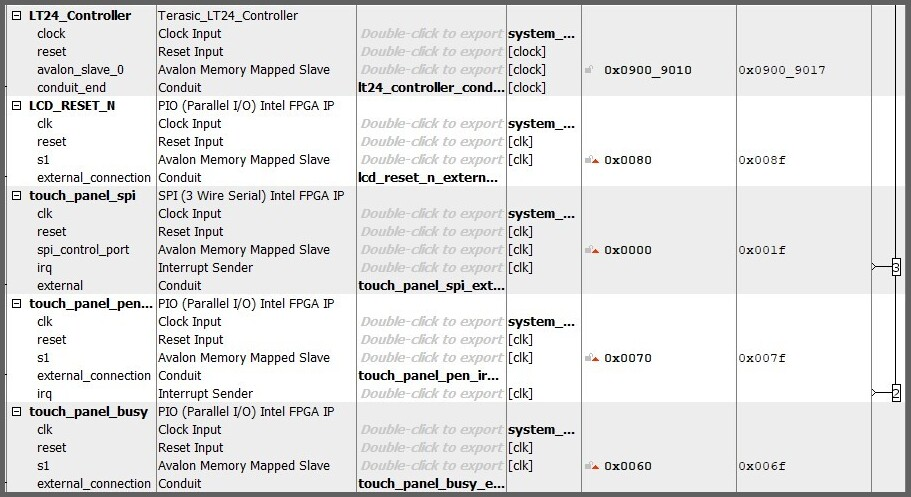
\includegraphics[width=1\linewidth]{img/LT24_modules.jpg}
    \caption{CPU LT24 modules instantiated}
    \label{fig:LT24_modules}
\end{figure}

\subsubsection{Floating-point operator module}

The floating-point operator module provides hardware support for floating-point arithmetic operations.

\begin{figure}[h!]
    \centering
    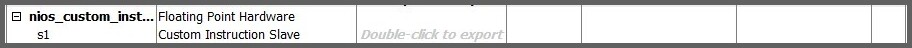
\includegraphics[width=1\linewidth]{img/floating_point_module.jpg}
    \caption{CPU floating-point operator module instantiated}
    \label{fig:floating_point_module}
\end{figure}

\newpage
\subsection{Timing analysis}

This section defines the physical root clocks entering the device and characterizes the internal clock trees synthesized by the Phase-Locked Loop (PLL) hardware macro. \\
These constraints ensure that the Static Timing Analysis engine can accurately verify setup and hold timing margins across all clock domains.

\subsubsection{Timing configuration file}

The provided Synopsys Design Constraints (SDC) code snippet establishes the fundamental timing environment for the FPGA design.

\vspace{1em}
\begin{lstlisting}[language=sdc, caption=Base clock settings for timing analyzer, label={lst:base_clock_settings}]
    create_clock    
        -name {altera_reserved_tck} 
        -period 100.000 
        -waveform { 0.000 50.000 } 
        [get_ports {altera_reserved_tck}]
    create_clock 
        -name {ADC_CLK_10} 
        -period 100.000 
        -waveform { 0.000 50.000 } 
        [get_ports {ADC_CLK_10}]
    create_clock    
        -name {MAX10_CLK1_50} 
        -period 20.000 
        -waveform { 0.000 10.000 } 
        [get_ports {MAX10_CLK1_50}]
                    
    derive_pll_clocks
\end{lstlisting}

\noindent
The base clocks settings present in \autoref{lst:base_clock_settings} represent physical, periodic signals routed from external oscillators on the board to specific input ports of the FPGA.

\begin{itemize}
    \item \texttt{altera\_reserved\_tck} \\
    is dedicated to the asynchronous JTAG Test Clock tap for hardware debugging. 

    \item \texttt{ADC\_CLK\_10} \\
    is the \(10\ \text{MHz}\) clock used to drive the controller of the LT24 touchscreen.
    
    \item \texttt{MAX10\_CLK1\_50} \\
    these serve as the primary external reference clocks feeding the internal logic and PLL inputs.

    \item \texttt{derive\_pll\_clocks} \\
    this command instructs Intel Quartus Prime to automatically detect internal PLL instances.

\end{itemize}

\noindent
Generated clocks represent signals derived from an existing master clock inside the FPGA, altered via frequency multiplication, division, or phase shifts.

\vspace{1em}
\begin{lstlisting}[language=sdc, caption=Generated clock settings for timing analyzer]
    create_generated_clock 
        -name {clk_dram_ext} 
        -source [get_pins{ u0|system_pll|sd1|pll7|clk[1] }] 
        [get_ports {DRAM_CLK}] 
    create_generated_clock  
        -name {u0|system_pll|sd1|pll7|clk[0]} 
        -source [get_pins{u0|system_pll|sd1|pll7|inclk[0]}] 
        -duty_cycle 50/1 -multiply_by 2 
        -master_clock {MAX10_CLK1_50} 
        [get_pins {u0|system_pll|sd1|pll7|clk[0]}] 
    create_generated_clock  
        -name {u0|system_pll|sd1|pll7|clk[3]} 
        -source [get_pins{u0|system_pll|sd1|pll7|inclk[0]}] 
        -duty_cycle 50/1 -multiply_by 1 
        -divide_by 5 -master_clock {MAX10_CLK1_50} 
        [get_pins{u0|system_pll|sd1|pll7|clk[3]}] 
\end{lstlisting}

\noindent
The paths originating from the switches and push-buttons were subsequently defined as asynchronous (unconstrained), while timing constraints were also specified for the paths driving the seven-segment displays and leds.

\vspace{1em}
\begin{lstlisting}[language=sdc, caption=Paths constraints for asynchronous buttons and leds on the board]
    set_false_path 
        -from [get_ports {SW[*] KEY[*]}] 
    set_false_path 
        -from [get_ports {LT24_ADC_*}] 
    set_false_path 
        -to [get_ports {HEX0[*] HEX1[*] HEX2[*] HEX3[*]
                        HEX4[*] HEX5[*] LEDR[*]}]
\end{lstlisting}

\noindent
Furthermore, based on the timing specifications provided in the corresponding datasheets, minimum and maximum output delays were defined for both the SDRAM interface and the JTAG Debug Module (USB Blaster). \\
The timing constraints for the JTAG Debug Module (USB Blaster) were derived using the forum \cite{altera_jtag_constraints_2026}. \\
For the LT24 display interface, since it is not directly synchronized to the system clock and all timing requirements are handled internally by a controller operating at \(10 \; \text{MHz}\), arbitrary minimum and maximum output delay values (\(1 \; \text{ns}\) in this implementation) were assigned relative to the clock signal. \\
In this case, verifying synchronization with the clock is sufficient to guarantee correct timing behavior, as the LT24 controller itself enforces the required interface timing.

\vspace{1em}
\begin{lstlisting}[language=sdc, caption=Paths constraints for SDRAM]
    set_input_delay 
        -add_delay -max -clock [get_clocks {clk_dram_ext}]  
        5.900 [get_ports {DRAM_DQ[*]}]
    set_input_delay 
        -add_delay -min -clock [get_clocks {clk_dram_ext}]  
        3.000 [get_ports {DRAM_DQ[*]}]
    set_output_delay 
        -add_delay -max -clock [get_clocks {clk_dram_ext}]
        1.600 [get_ports {DRAM_ADDR[*]}]
    set_output_delay 
        -add_delay -min -clock [get_clocks {clk_dram_ext}]  
        -0.900 [get_ports {DRAM_ADDR[*]}]
\end{lstlisting}

\begin{lstlisting}[language=sdc, caption=Paths constraints for LT24 module]
    set_output_delay 
        -add_delay  
        -clock [get_clocks {u0|system_pll|sd1|pll7|clk[3]}]  
        1.000 [get_ports {LT24_*}]
\end{lstlisting}

\begin{lstlisting}[language=sdc, caption=Paths constraints for JTAG Debug Module (USB Blaster)]
    set_input_delay 
        -add_delay -max 
        -clock [get_clocks {altera_reserved_tck}]  
        10.000 [get_ports {altera_reserved_tdi}]
    set_input_delay 
        -add_delay -min 
        -clock [get_clocks {altera_reserved_tck}]  
        2.000 [get_ports {altera_reserved_tdi}]
    set_input_delay 
        -add_delay -max 
        -clock [get_clocks {altera_reserved_tck}]  
        10.000 [get_ports {altera_reserved_tms}]
    set_input_delay 
        -add_delay -min 
        -clock [get_clocks {altera_reserved_tck}]  
        2.000 [get_ports {altera_reserved_tms}]
    set_output_delay 
        -add_delay -max 
        -clock [get_clocks {altera_reserved_tck}]  
        10.000 [get_ports {altera_reserved_tdo}]
    set_output_delay 
        -add_delay -min 
        -clock [get_clocks {altera_reserved_tck}]  
        2.000 [get_ports {altera_reserved_tdo}]  
\end{lstlisting}

\newpage
\subsubsection{Maximum Frequency Report}
The timing analyzer uses the library of the FPGA macro-cells to verify that the timing constraints are respected for both the slow and fast models.\\
The slow model is used to check the maximum frequency of the clock sources (at a temperature of \(85^\circ C\) worst case) and the setup timing constraints.\\
The fast model is used to verify that hold time violations do not occur (at a temperature of \(0^\circ C\) best case).

\begin{figure}[h!]
    \centering
    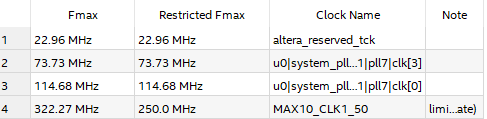
\includegraphics[width=\textwidth]{img/timing_analyzer_fmax.png}
    \caption{Maximum frequency Timing analyzer report}
    \label{fig:timing_analyzer_fmax}
\end{figure}

\begin{itemize}
    \item \texttt{Internal System Clock (clk[0])} \\
    The Nios II CPU and all associated modules meet the timing requirements. Since the maximum achievable frequency ($114.68 \; \text{MHz}$) exceeds the target frequency ($100 \; \text{MHz}$), the system operates with positive timing slack.

    \item \texttt{LT24 Display Clock (clk[3])} \\
    Although the internal logic could theoretically operate up to $73.73 \; \text{MHz}$, only $10 \; \text{MHz}$ is required for the LT24 interface. As specified in the LT24 datasheet, higher frequencies may cause data corruption; therefore, the clock frequency is kept at or below $10 \; \text{MHz}$ despite the available timing margin.

    \item \texttt{JTAG Debug Clock (altera\_reserved\_tck)} \\
    The timing analysis confirms compliance with the required $10 \; \text{MHz}$ operating frequency.
\end{itemize}

\noindent
\textit{Note: The timing analyzer indicates that while the internal silicon routing from this clock pin is capable of supporting frequencies up to $322.27 \; \text{MHz}$, the physical I/O buffer architecture of the MAX 10 device imposes a hard limit at $250.0 \; \text{MHz}$. \\
This limitation is due to the electrical switching capability of the I/O transistors, which cannot reliably toggle beyond this frequency. \\
However, this constraint is not a concern in practice, since the operating frequency of $50 \; \text{MHz}$ is well below both the I/O limit ($250 \; \text{MHz}$) and the internal routing limit ($322.27 \; \text{MHz}$), resulting in a substantial safety margin for this clock domain. Quartus therefore caps the reported maximum frequency at $250 \; \text{MHz}$ to prevent unrealistic external clock assumptions in future design iterations.}

\newpage

\subsubsection{Hold and Setup Time Slack Report}
The timing analyzer evaluates the setup and hold slack for each clock domain to ensure correct data latching and prevent metastability. \\
The setup analysis checks that the data arrives at the destination register before the next clock edge, whereas the hold analysis ensures the data remains stable long enough after the clock edge to be properly sampled. \\
As shown in the \autoref{fig:timing_slack_reports}, all clock domains exhibit positive slack, confirming that the design fully meets all timing requirements under both worst-case and best-case operating conditions.

\begin{figure}[h!]
    \centering
    \begin{subfigure}[b]{0.48\textwidth}
        \centering
        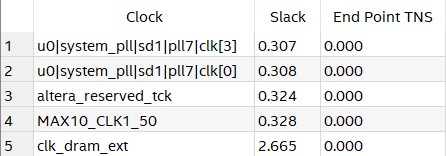
\includegraphics[width=\textwidth]{img/hold_summary.jpg}
        \caption{Hold summary report}
        \label{fig:hold_summary}
    \end{subfigure}
    \hfill
    \begin{subfigure}[b]{0.48\textwidth}
        \centering
        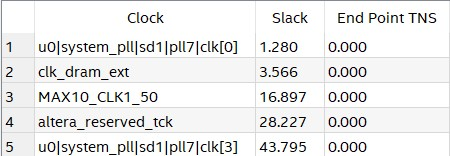
\includegraphics[width=\textwidth]{img/setup_summary.jpg}
        \caption{Setup summary report}
        \label{fig:setup_summary}
    \end{subfigure}
    \caption{Hold and Setup slack Timing analyzer reports}
    \label{fig:timing_slack_reports}
\end{figure}

\begin{itemize}
    \item \texttt{Internal System Clock (clk[0])} \\
    The system clock meets both timing constraints comfortably. It presents a worst-case hold slack of $0.308 \; \text{ns}$ and a setup slack of $1.280 \; \text{ns}$. The positive margins ensure stable synchronous operations within the Nios II CPU and its peripherals.

    \item \texttt{LT24 Display Clock (clk[3])} \\
    The clock domain dedicated to the LT24 display interface reports a hold slack of $0.307 \; \text{ns}$ and a substantial setup slack of $43.795 \; \text{ns}$. This significant setup margin is a direct consequence of the relaxed operating frequency ($10 \; \text{MHz}$) compared to the maximum frequency supported by the internal logic routing.

    \item \texttt{External DRAM Clock (clk\_dram\_ext)} \\
    The external memory clock domain exhibits high robust timing margins, showing a hold slack of $2.665 \; \text{ns}$ and a setup slack of $3.566 \; \text{ns}$. This ensures reliable data transfer with the external SDRAM chip.

    \item \texttt{System Input Clock (MAX10\_CLK1\_50)} \\
    The $50 \; \text{MHz}$ main input clock shows a hold slack of $0.328 \; \text{ns}$ and a setup slack of $16.897 \; \text{ns}$, confirming safe propagation of the external reference clock into the internal PLL structures.

    \item \texttt{JTAG Debug Clock (altera\_reserved\_tck)} \\
    The JTAG test clock complies with the constraints, reporting a hold slack of $0.324 \; \text{ns}$ and a setup margin of $28.227 \; \text{ns}$.
\end{itemize}

\newpage
\subsection{Resource Usage}
\label{sssec:hw_footprint_chpl}

Compared to all the resources available on the chip, the total logic elements used are only \(17\%\) of the total, and the total memory bits used are \(11\%\), as shown in \autoref{fig:resorces_usage}. \\
Furthermore only 16 of the 288 embedded multipliers and one of the four internal PLL.

\begin{figure}[h!]
    \centering
    \begin{subfigure}[t]{0.45\textwidth}
        \centering
        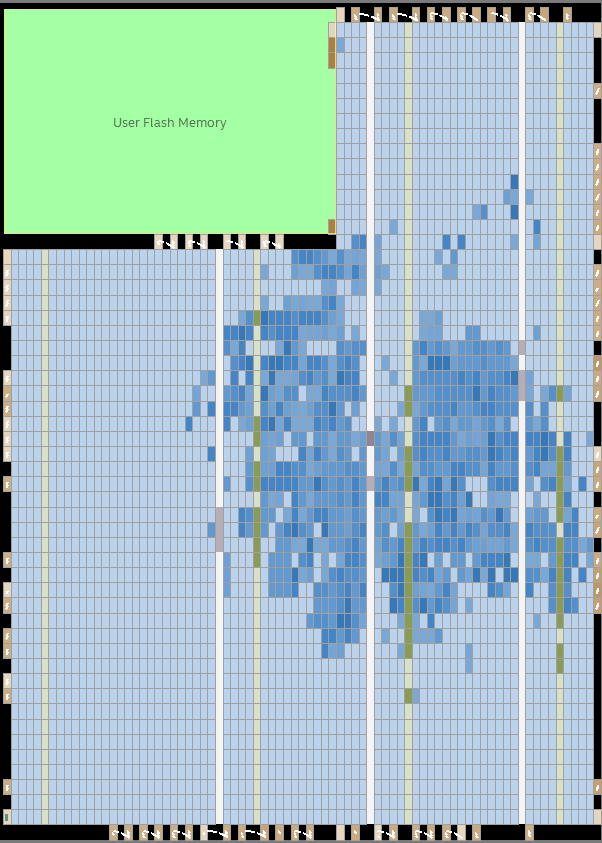
\includegraphics[width=\textwidth]{img/chip_planner_view.png} 
        \caption{Hardware-Footprint on Chip Planner}
        \label{fig:chip_planner_view}
    \end{subfigure}
    \hfill 
    \begin{subfigure}[t]{0.45\textwidth}
        \centering
        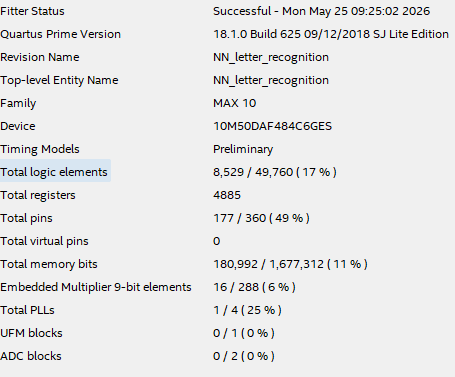
\includegraphics[width=\textwidth]{img/fitter_summary.png} 
        \caption{Fitter summary hardware used}
        \label{fig:fitter_summary}
    \end{subfigure}
    
    \caption{FPGA resources usage}
    \label{fig:resorces_usage}
\end{figure}
